% !TEX root = da.tex

\subsection{The base geodesic flow kernel (GFK)}  \label{sGFK}


\begin{figure*}[t]
\centering
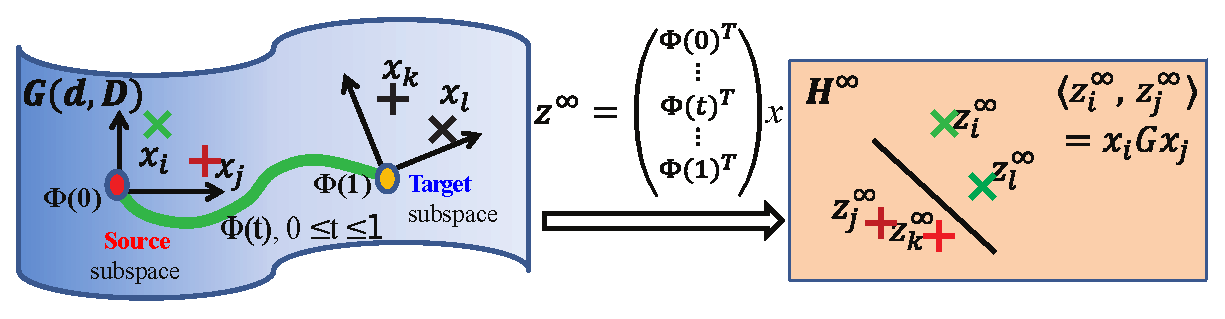
\includegraphics[width=0.9\columnwidth]{fig/fConcept4}
\caption{Main idea of our geodesic flow kernel (GFK). The source and target domains are embedded in a Grassmann manifold, which is a collection of all $d$-dimensional subspaces of $\R^\cst{D}$. We connect the two subspaces of the two domains by a continuous geodesic flow $\mat{\Phi(t)}$. After projecting a data point $\vct{x}$ to this flow, we arrive at an infinitely dimensional feature vector $\vct{z}^\infty\in\mathcal{H}^\infty$ which encapsulates incremental changes from the source subspace to the target subspace. As a result, the inner product between two such vectors ``averages out'' the domains' idiosyncrasies and can be analytically computed in a closed form. (best viewed in color)}
\label{fConceptGFK}
\end{figure*}

\eat{
\subsection{Main idea} \label{sGFK-main}
Our approach  follows broadly the theme of identifying the \emph{shared representation} between different domains~\cite{bendavid07domain}. Intuitively, we seek a feature space such that when data points are projected into this space, the source domain is similar to the target domain. How to define and quantify shared characteristics entails careful examination of our intuition on what type of representation facilitates adaptation. For example, in the part-of-speech (POS) task of tagging words into different syntactic categories \cite{BlitzerEMNLP06Domain}, the idea is to extract shared patterns from  auxiliary classification tasks that predict ``pivot features'', frequent words which are themselves discriminative in both domains.  While sensible for language processing tasks, typical histogram based features of low-level visual descriptors do not have the benefits of pivot ``visual words'' --- in general, no single feature dimension from a particular histogram bin is discriminative enough to differentiate visual categories.

On the other hand, many visual data {are} assumed to lie in low-dimensional subspaces.  Given data from two domains, \emph{how can we exploit the subspaces in these datasets, which can be telltale cues in revealing the underlying difference and commonness between the domains?}
}

GFKs serve as the basis for the second stage of our approach --- using landmarks to discriminatively combine multiple GFKs for classifying the target data. Our main idea behind GFK is to {\em implicitly} construct  a feature space that aggregates information on the source domain $ \src$, the target $\tgt$, and ``phantom'' domains interpolating between those two. In particular, the phantom domains represent incremental changes in the geometric and statistical properties between the two domains.

While each of the domains is represented with a subspace, the inner products in $\mathcal{H}^\infty$ are defined to integrate over an infinite number of such subspaces. Intuitively, this integration averages out domain-specific idiosyncrasies and computes similarity measures that are insensitive to domain mismatch. Equivalently, the inner products give rise to a kernel function that defines the kernel mapping from the original feature space to a domain-invariant feature space. Fig.~\ref{fConceptGFK} sketches the main idea.

In the following, we start by reviewing some basic notions of Grassmann manifolds. The subspaces of the source and target domains are represented as two points on one such manifold.  Furthermore, the phantom domains correspond to the points on the geodesic path connecting those two points. 

\subsubsection{Modeling domains on Grassmann manifold}
In statistical modeling, we often assume data can be embedded in a
low-dimensional linear subspace. For example, principal component
analysis (PCA) identifies the subspace where the variances of the
embedded data are maximized. It is convenient to refer to a subspace with its  basis $\mat{P}\in
\R^{\cst{D}\times \cst{d}}$, where $\cst{D}$ and $\cst{d}$ are the dimensions of the data and subspace, respectively. \eat{For
PCA, the basis is then the top $\cst{d}$ eigenvectors of the data's
covariance matrix.}   The collection of all $\cst{d}$-dimensional
subspaces form the Grassmannian $\mathbb{G}(\cst{d},\cst{D})$, a
smooth Riemannian manifold on which we can define  geometric, differential, and probabilistic structures.

As an intuitive example of how manifolds can help us tackle domain adaptation, imagine that we compute the subspaces of the datasets for the $ \src$ and $\tgt$ domains and map them to two points on a Grassmannian.  Intuitively, if these two points are close by, then the two domains could be similar in the distribution of their data. Thus, a source $\src$-trained classifier is likely to work well on the target $\tgt$.

However, \emph{what if these two domains are far apart on the manifold?} For example, suppose two datasets of car images with large differences in poses are placed far apart on the manifold.
We aim to use intermediate subspaces to learn domain-invariant features for adaptation.
Specifically, the intermediate subspaces would capture statistics of car images under poses interpolated between the source and the target domains. Being informed of all these different subspaces from the same category, the learning algorithms might be able to extract features that are less sensitive to variations in pose.
To this end, we will use the geodesic flow path to connect the two domains, where every point on this flow path is an intermediate subspace.


\subsubsection{Defining the geodesic flow kernel (GFK)}
\label{sGFK-detail}
Our approach consists of the following steps: i) determine the optimal dimensionality of the subspaces to embed domains; ii) construct the geodesic flow; iii) compute the geodesic flow kernel; iv) use the kernel to construct a classifier with the labeled data of the source domain. We defer describing step i) to the next section and focus on steps ii) and iii). For step ii), we state only the main computational steps; the detailed derivation can be found in \cite{gopalan2011domain} and references therein. Step iv) is omitted for brevity, as it is the same as constructing any other kernel-based classifiers.

{\bf Construct geodesic flow.}  Let $\srcbase, \tgtbase \in \R^{\cst{D}\times\cst{d}}$ denote the two sets of basis of the subspaces for the source and target domains, respectively. Let $\srccomp \in \R^{\cst{D}\times (\cst{D-d})}$ denote the orthogonal complement to $\srcbase$, namely $\srccomp\T\srcbase = \mat{0}$. Using the canonical Euclidean metric for the Riemannian manifold, the geodesic  flow is parameterized as $\mat{\Phi}: t\in [0, 1]\rightarrow \mat{\Phi}(t) \in {G}(\cst{d},\cst{D})$ under the constraints that $\mat{\Phi}(0)$ is the subspace of the source domain and $\mat{\Phi}(1)$ be the subspace of the target.  For other $t$, we have
\begin{equation}
\mat{\Phi}(t) = \srcbase\mat{U}_1 \mat{\Gamma}(t) -  \srccomp\mat{U}_2 \mat{\Sigma}(t),
\label{eFlow}
\end{equation} %Combining the two,  $[ \srcbase\ \  \srccomp]$ is the complete basis of $\R^{\cst{D}}$.
where $\mat{U}_1 \in \R^{\cst{d}\times\cst{d}}$ and $\mat{U}_2 \in \R^{(\cst{D-d})\times\cst{d}}$  are orthonormal matrices. They are given by the following pair of (generalized) SVDs,
\begin{equation}
\srcbase\T\tgtbase = \mat{U}_1 \mat{\Gamma} \mat{V}\T,\ \ \ \srccomp\T\tgtbase = - \mat{U}_2 \mat{\Sigma}\mat{V}\T\ .
\label{eSVD}
\end{equation}
$\mat{\Gamma}$ and $\mat{\Sigma}$ are $\cst{d}\times\cst{d}$ diagonal matrices with the diagonal elements of $\cos\theta_i$ and $\sin\theta_i$, respectively.  In particular, $\theta_i$ are called the principal angles between $\srcbase$ and $\tgtbase$, measuring
 the degree by which subspaces ``overlap''. %They are instrumental to our approaches for choosing the optimal dimensionality . We come back to them  in later sections.
%Eigenvectors in $\mat{U}_1$, $\mat{U}_2$ and $\mat{V}$ are called canonical bases. \FS{Check the definition on this.. A bit off, I think}.
Moreover, $\mat{\Gamma}(t)$ and $\mat{\Sigma}(t)$ are diagonal matrices whose elements are $\cos(t\theta_i)$ and $\sin(t\theta_i)$ respectively.

{\bf Compute the geodesic flow kernel (GFK).}  The geodesic flow parameterizes how the source domain smoothly changes to the target domain.  Consider the subspace $\mat{\Phi}(t)$ for $t\in (0,1)$ and compute $\mat{\Phi}(t)\T\vct{x}$, i.e., the projection of a feature vector $\vct{x}$ into this subspace. If $\vct{x}$ is from the source domain and $t$ is close to 1, then the projection  will  appear as if it is likely coming from the target domain, and conversely for $t$ close to 0. Thus, using the projections to the subspaces ($\mat{\Phi}(t)$, $t\in[0,1]$) to build a classifier  would result in a model using a set of features that are characteristic  of both domains. Hence, this classifier would likely perform well on the target domain.

%\FS{This argument is a bit faulty: a classifier, if cross-validated on the source data, will choose Ps automatically and ignore all other features from the flow. This might be the reason that Gopalan's method cannot be used directly with linear discriminant etc. Nevertheless, we need to find a way to defend this potential critique from reviewers. See below...from "Another benefits".}

Which (or which set of) $t$ should we use then?  Our answer is surprising at the first glance: \emph{all of them}! Intuitively, by expanding the original features with projections into \textbf{all} subspaces, we force a measurement of similarity (as we will be using inner products to construct classifiers) that is robust to any variation that leans either toward the source or towards the target or in between. In other words, the net effect is a representation that is insensitive to idiosyncrasies in either domain. 
%We will discuss first how to avoid choosing $\cst{K}$ and $\cst{M}$.  Then in the next section, we will describe how to choose $\cst{d}$ optimally. Our first step appears to be counter-intuitive. Instead of using smaller $\cst{K}$ thus reducing the dimensionality of augmented feature space, we increase $\cst{K}$ to infinity by sampling every point on the curve.

Computationally, however, we cannot use this representation explicitly.  Nevertheless, we next show that there is no need to actually compute, store, and  manipulate the infinitely many projections.

For two original $\cst{D}$-dimensional feature vectors $\vct{x}_i$ and $\vct{x}_j$, we compute their projections into $\mat{\Phi}(t)$ for a continuous $t$ from $0$ to $1$ and concatenate all the projections into infinite-dimensional feature vectors $\vct{z}_i^\infty$ and $\vct{z}_j^\infty$. The inner product between them defines our geodesic flow kernel (GFK),
\begin{equation} \label{eDAK}
\langle \vct{z}_i^\infty, \vct{z}_j^\infty \rangle= \int_0^1 (\mat{\Phi}(t)\T\vct{x}_i)\T(\mat{\Phi}(t)\T\vct{x}_j)\ dt = \vct{x}_i\T \kernel\vct{x}_j,
\end{equation}
where $\mat{G}\in \R^{\cst{D}\times\cst{D}}$ is  positive semidefinite. This  is precisely the ``kernel trick'', where a kernel function induces inner products in an infinite-dimensional feature space. The matrix $\kernel$ can be computed in closed-form from previously defined matrices:
\begin{equation}
\kernel = [ \srcbase\mat{U}_1 \ \  \srccomp\mat{U}_2 ] \left[\begin{aligned}
\mat{\Lambda}_1 & & \mat{\Lambda}_2\\
\mat{\Lambda}_2 & & \mat{\Lambda}_3\end{aligned} \right]\left[\begin{aligned}
\mat{U}_1\T\srcbase\T\\
\mat{U}_2\T\srccomp\T
\end{aligned}\right]
\label{eGFKDef}
\end{equation}
where $\mat{\Lambda}_1$ to $\mat{\Lambda}_3$ are diagonal matrices, whose diagonal elements are
\begin{equation}
\lambda_{1i} = 1+{\sin(2\theta_i)}/{(2\theta_i)},  \; \lambda_{2i} = {(\cos(2\theta_i)-1)}/{(2\theta_i)},  \; \lambda_{3i} = 1-{\sin(2\theta_i)}/{(2\theta_i)}. \notag
\end{equation}
Detailed derivations are given in the appendix of~\cite{GongIJCV14Learning}, where we also justify the rationale behind GFK: How exactly does GFK reduce the discrepancy across domains? At the high level, 
it leads to measuring {\em distances} between data points in a way that is insensitive to domains. The empirical studies there reveal that the subspaces induced by GFK best satisfy two desirable properties \emph{simultaneously} for the distance measures: minimal distortions to the distances in the original source and target domains, \emph{and} matching how distances of the two domains are distributed. %The observations are echoed by the superior performance of GFK in benchmark problems, reported in section~\ref{sExp}.


{\bf Extract domain-invariant feature space.}  The kernel $\mat{G}$ can be plugged into any kernelized classifiers (e.g., SVMs). Additionally, we can extract from it an equivalent  finite-dimensional domain-invariant feature space. Let $\mat{L}$ be $\mat{G}$'s square root: $\mat{L}\T\mat{L} = \mat{G}$. The domain-invariant feature space is given by the mapping $\vct{x} \rightarrow  \vct{z} = \mat{L}\vct{x}$, such that $\vct{z}_i\T\vct{z}_j = \vct{x}_i\T\mat{G}\vct{x}_j$.  This explicit feature representation is convenient for constructing other types of classifiers that do not depend on inner products.


The closed-form expression of GFK is convenient to use and does not depend on user-selected parameters (e.g., the bandwidth in Gaussian RBF kernels). In practice, we need to choose the dimension $\cst{d}$ of the subspaces. We  show next how to automatically infer this hyperparameter from the data, thus making the proposed method fully automatic and free of tuning any hyperparameters.

\eat{
\subsection{Automatic inference of subspace dimension $\cst{d}$}
\label{sDim}
The intuition behind our approach of automatically inferring the dimension $\cst{d}$ of the subspaces is to align as much as possible the subspaces of the source and target domains.  To this end, we develop a subspace disagreement metric (SDM). We first compute the PCA subspaces of the two datasets, $\srcpca$ and $\tgtpca$. We also combine the datasets into one and compute its subspace\, $\stpca$. Intuitively, if the two datasets are similar, then all three subspaces should not be too far away from each other on the Grassmannian. SDM captures this notion and is defined as,
\begin{equation}
\mathcal{D}(\cst{d}) =  0.5 \left[\sin\alpha_\cst{d} + \sin\beta_\cst{d} \right],
\label{eDim}
\end{equation}
where $\alpha_\cst{d}$ denotes the $\cst{d}$-th principal angle (cf.\ eq.~(\ref{eAngles})) between $\srcpca$ and $\stpca$ and $\beta_\cst{d}$ between $\tgtpca$ and $\stpca$. The quantity $\sin\alpha_\cst{d}$ or $\sin\beta_\cst{d}$ is called the minimum correlation distance \cite{hamm2008grassmann} in the Grassmannian.% between the two subspaces.

Note that $\mathcal{D}(\cst{d})$ is  at most 1. A small value indicates that both $\alpha_\cst{d}$ and $\beta_\cst{d}$ are small, thus $\srcpca$ and $\tgtpca$ are aligned (at the $\cst{d}$-th dimension).  At its maximum value of 1, the two subspaces have orthogonal directions (i.e., $\alpha_d = \beta_d=\pi/2$). In this case, domain adaptation will become difficult as variances captured in one subspace would not be able to transfer to the other subspace.

To identify the optimal $\cst{d}$, we adopt a greedy strategy:
\begin{equation}
\cst{d}^* = \min  \{\cst{d}|  \mathcal{D}(\cst{d}) = 1\}.
\label{eDim2}
\end{equation}
In words, the optimal dimension $\cst{d}^*$ should be as high as possible (to preserve variances in the source domain for the purpose of building good classifiers) but should not be so high that the two subspaces start to have orthogonal directions.
}





\eat{
\subsection{Reducing domain discrepancy with the GFK}
\label{sGFKAnalysis}

Building on the general intuitions described above, we now more formally justify the rationale behind the GFK.  How exactly does GFK reduce the discrepancy across domains? The definition of the kernel in eq.~(\ref{eDAK}) provides several clues. In particular, we will show in the following that the proposed kernel construction leads to measuring distances between data points in a way that is insensitive to domains.

To start with, consider that we would like to use a nearest neighbor classifier on both the source and the target domains in an ideal domain-invariant feature subspace $\mathcal{F}$, parameterized by its basis $\mat{F}$.  What properties do we desire for the subspace $\mathcal{F}$? In what follows, we describe two such properties which are strongly correlated with empirical evidence in supporting using the GFK for deriving domain-invariant features.

At the foremost, we would like $\mathcal{F}$ to preserve distances between data points measured within the source domain's subspace. Namely,
\begin{equation}
\| \mat{F}\T\vct{x}_i - \mat{F}\T\vct{x}_j \|_2^2  - \| \srcbase\T\vct{x}_i - \srcbase\T\vct{x}_j \|_2^2 \approx 0,
\end{equation}
for points $\vct{x}_i, \vct{x}_j \in \src$. This is analogous to the central ideas of many manifold learning algorithms to preserve distances.  Similarly, for a pair of data points $\vct{x}_m$ and $\vct{x}_n$ from the target domain $\tgt$, we would like
\begin{equation}
\| \mat{F}\T\vct{x}_m - \mat{F}\T\vct{x}_n \|_2^2- \| \tgtbase\T\vct{x}_m - \tgtbase\T\vct{x}_n \|_2^2 \approx 0.
\end{equation}
Along the geodesic flow eq.~(\ref{eFlow}), if we select the subspace $\mat{F} = \mat{\Phi(t)}$ with  $t \ll 1$, the distance-preserving condition for the source domain is easy to be satisfied as $\mat{F}$ would be close to $\srcbase$. However, such $\mat{F}$ would distort the distance-preserving condition for the target domain significantly as $\mat{F}$ would be very different from $\tgtbase$. Conversely, for $t \approx 1$, the selected subspace $\mat{F}$ on the flow will preserve distances in the opposite way.

The ``right'' choice is then to balance the averaged distortion ratios (i.e., distortions divided by distances) for each domain and select an intermediate point on the flow. While feasible in theory (for instance, by minimizing a properly constructed objective function over $t$), an alternative approach is to use \emph{all subspaces}, as in the derivation of our GFK. The intuition is  ``to average out'': for any $t$, if the subspace $\mat{\Phi}(t)$ preserves the distances for the source domain better than the target domain, then for $(1-t)$, the converse is true. In other words, if uniformly sampling the flow, the expected distortion is the same for both domains --- we are not favoring any particular one of them. More precisely, this subspace will give rise to the following distance function
\begin{equation}
\| \mat{F}\T\vct{x} - \mat{F}\T\vct{x}' \|_2^2 = (\vct{x} - \vct{x}')\T\int_t \mat{\Phi}(t)\T\mat{\Phi}(t) dt\, (\vct{x} - \vct{x}'),
\end{equation}
which is precisely defined in terms of our GFK.

\begin{table}
\centering
\caption{Distortion ratios (in \%) to distances computed within the source and target domains, using 4 subspaces}
\label{tDistPreserve}
\begin{tabular}{|c|c|c|c|c|}\hline
Domain pairs & \PCAs & \PCAt & \PCAst & \GFK \\ \hline
\amazon - \caltech &  8.78 & 7.71 & 5.48 & 6.18 \\ \hline
\amazon - \dslr & 19.9  & 17.3 & 15.9 & 13.2 \\ \hline
\amazon - \webcam & 15.5 & 14.0 & 11.8 & 10.8 \\ \hline
\caltech - \dslr & 14.1 & 16.3 & 12.1 & 11.1 \\ \hline
\caltech - \webcam & 15.5 & 14.8 & 11.0 & 10.9 \\ \hline
\dslr - \webcam & 15.7 & 13.7 & 10.4 & 10.6 \\ \hline\hline
Average & 14.9 & 14.0 & 11.1 & \textbf{10.5} \\ \hline
\end{tabular}
\end{table}

To help illustrate this point, Table~\ref{tDistPreserve} reports the averaged distortion ratios computed within the source and target domains, using four different subspaces: the PCA subspace of the source (\PCAs), the PCA subspace of the target (\PCAt), the PCA subspace of merging the source and the target (\PCAst), and the subspace induced by our GFK (\GFK). We report results on six different pairs of source and target domains (all used in our experimental studies for domain adaptation in section~\ref{sExp}). The subspace by our GFK attains the smallest distortion.

The second property we desire for $\mathcal{F}$ is closely related to our goal of using the source labeled data to classify the target unlabeled data. Intuitively, if we use $\mat{F}$ to  measure pairwise distances within each domain, then those two sets of distances should be similarly distributed. Otherwise, the data instances in the target domain will not be classified as effectively as the instances in the source domain. This is especially true if data follows the assumption of discriminative clustering --- all instances from the same class form a tight cluster and different clusters tend to be apart from each other~\cite{shi2012}.

Fig.~\ref{fGFKKLDistance} displays the histograms of those pairwise distances computed using several subspaces.   The source domain is the \amazon\ dataset and the target domain is the \webcam\ dataset (for a detailed description of these datasets, please refer to section~\ref{sExp}). We see that the subspace corresponding to GFK brings the source and the target domains closest.  Table~\ref{tGFKKLDistance} quantitatively confirms the outcome; we report the symmetric KL divergence between those histograms for the same six pairs of source and target domains as in Table~\ref{tDistPreserve}. Clearly, GFK is able to attain the smallest divergences.

\begin{figure}
\centering
\includegraphics[width=0.45\columnwidth]{fig/fAWKLDistPCAs}
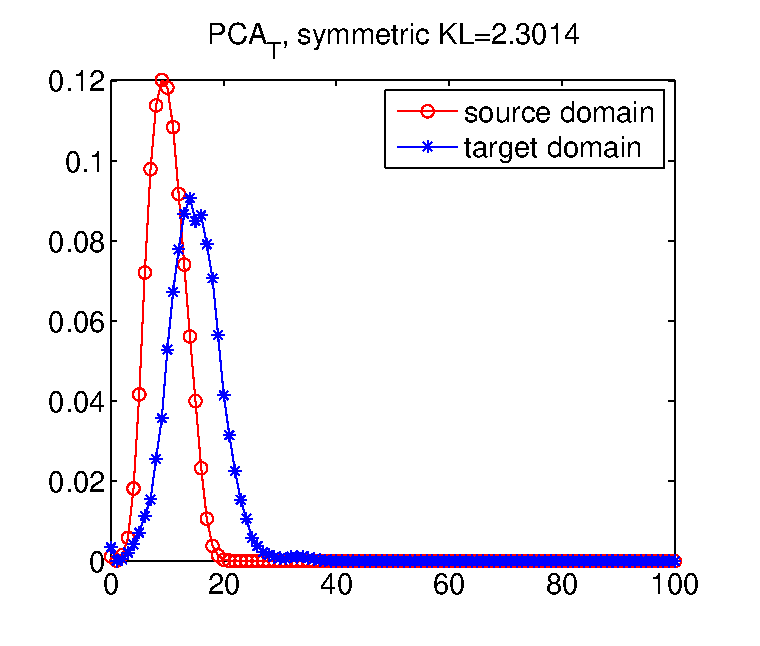
\includegraphics[width=0.45\columnwidth]{fig/fAWKLDistPCAt}\\
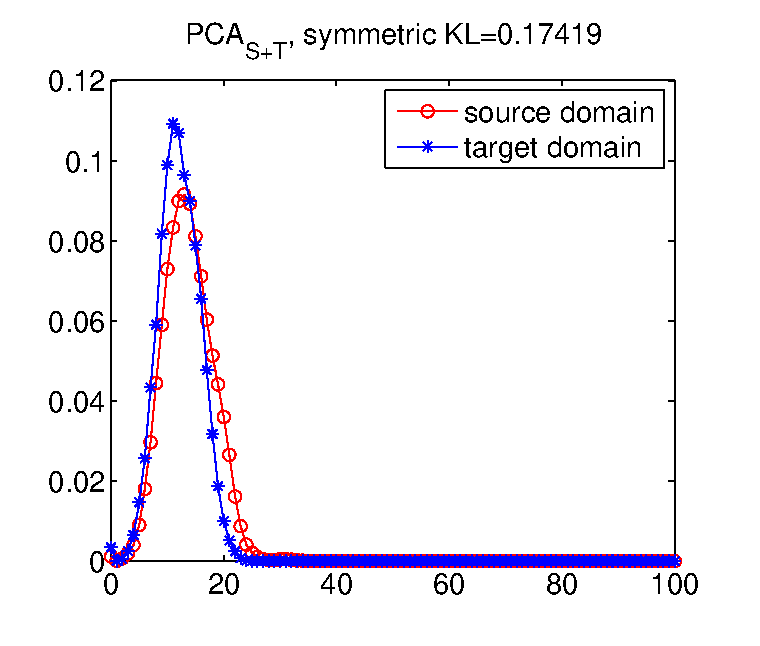
\includegraphics[width=0.45\columnwidth]{fig/fAWKLDistPCAst}
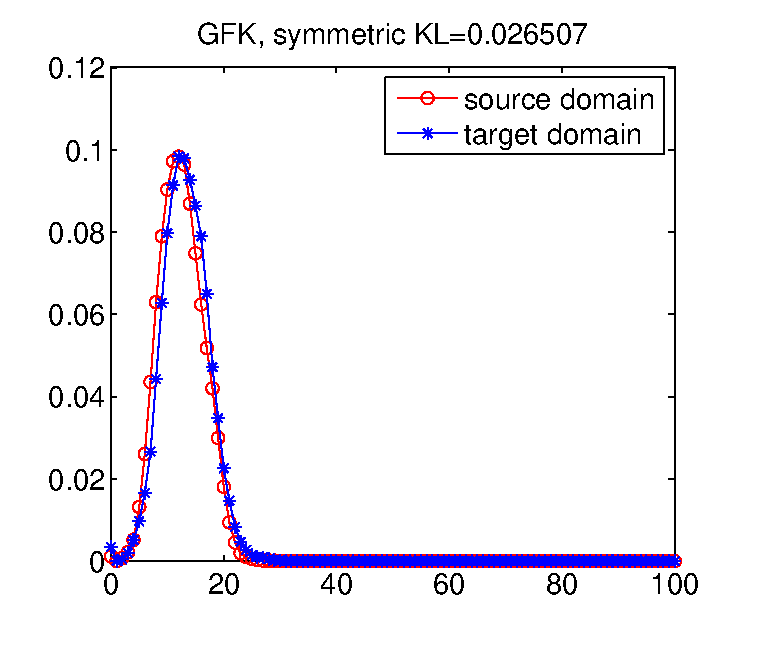
\includegraphics[width=0.45\columnwidth]{fig/fAWKLDistGFK}
\caption{Histograms of pairwise distances within each domain where the distances are calculated within four different subspaces. GFK induces  a subspace such that the difference between the source's histogram and the target's is the smallest.}
\label{fGFKKLDistance}
\end{figure}

\begin{table}
\centering
\caption{Symmetric KL divergences between the histograms of pairwise distances across two domains}
\label{tGFKKLDistance}
\begin{tabular}{|c|c|c|c|c|}\hline
Domain pairs & \PCAs & \PCAt & \PCAst & \GFK \\ \hline
\amazon - \caltech &  0.413 & 0.445 & 0.014 & 0.012 \\ \hline
\amazon - \dslr & 2.145 & 7.411 & 0.734 & 0.33 \\ \hline
\amazon - \webcam & 1.048 & 2.301 & 0.174 & 0.027 \\ \hline
\caltech - \dslr & 1.026 & 2.488 & 0.587 & 0.138 \\ \hline
\caltech - \webcam & 1.747 & 2.188 & 0.347 & 0.178 \\ \hline
\dslr - \webcam & 2.884 & 0.808 & 0.009 & 0.089 \\ \hline\hline
Average & 1.544 & 2.607 & 0.311 & \textbf{0.129} \\ \hline
\end{tabular}
\end{table}


Combining the results in Table~\ref{tDistPreserve} and~\ref{tGFKKLDistance}, we find that the GFK leads to a subspace that best satisfies the two desirable properties \emph{simultaneously}: minimal distortions to distances \textbf{and} matching how distances are distributed. This empirical evidence strongly supports the GFK as a method to extract domain-invariant features. This support is echoed by the superior performance of GFK in benchmark problems, reported in section~\ref{sExp}.
}



\subsubsection{GFK as a standalone approach to unsupervised domain adaptation}
We note that GFK entails domain-invariant features, since it ``averages out'' the domain idiosyncrasies by the intergation over the geodesic flow. As a result, we are able to directly use it to solve the unsupervised domain adaptation problem, in addition to employing it to build other algorithms (e.g., the landmark based method in the next section). Concretely, we  i) determine the optimal dimensionality of the subspaces either by the subspace disagreement measure~\cite{GongCVPR12Geodesic} or cross-validation; ii) compute the geodesic flow kernel $\mat{G}$ using the subspaces eq.~(\ref{eGFKDef}); iii) use the kernel to construct a classifier with  the labeled data, either using a kernelized classifier which requires only the inner products defined by the kernel matrix $\mat{G}$ or using the invariant features $\mat{L}\vct{x}$ in any other types of classifiers.% Experiments on visual object recognition (see section~\ref{eExp}) verify the effectiveness of GFK for solving unsupervised domain adaptation.% in the visual object recognition tasks. 
\newline \newline
{\bf Remark.} Gopalan \emph{et al.}'s work is the closest to our GFK approach in spirit \cite{gopalan2011domain}. They have also explored the idea of using geodesic flows to derive intermediate subspaces that interpolate between the source and target domains. A crucial difference from ours is that they sample a \emph{finite} number of subspaces and stack these subspaces into a very high-dimensional projection matrix. As such, the dimension of their features needs to be reduced. This extra step, unfortunately, might introduce modeling errors and practical challenges. For instance, it is not clear how to choose the subspace sampling rate or the right feature dimension after reduction. %and whether the dimension reduction method used there necessarily helps classification.

\eat{
In stark contrast, GFK is both conceptually and computationally simpler and eliminates the need to tune many hyper-parameters as by Gopalan \emph{et al.}'s approach. In particular, our kernel is in closed form, and computing it involves simple matrix algebra for example singular value decomposition. We have devised a fully automatic procedure, which is lacking in Gopalan \emph{et al.}'s work,  to choose the optimal dimensionality of the subspaces~\cite{GongCVPR12Geodesic}. {We also note that Zheng {\it et al.} proposed the same kernel, albeit independently and almost simultaneously~\cite{zheng2012grassmann}, though they did not offer an automatic procedure to determine the dimensions of the subspaces.}
}
